\documentclass[aspectratio=169]{beamer}
\usepackage[utf8]{inputenc}
\usepackage{tikz}
\usepackage{tikz-cd}
\usepackage{tikz-layers}
\usepackage{pifont}
\usepackage{pgfpages}
\usepackage{pgfplots}
\usepackage{graphicx}
\usepackage[export]{adjustbox}
\usepackage{qrcode}
\usepackage{caption}
\usepackage{minted}
\usetikzlibrary{decorations.pathreplacing}

\usetheme{drgtheme}

%setup cover page variables
\title{MAC 233: Arduino Introduction}
\author{
    Dr Dan Brennan
}
\institute[UoS-DRG]{
    School of Mechanical, Aerospace, and Civil Engineering,\\
    University of Sheffield, UK
}
\date{MAC 233: \hspace{0.1em}\textbf{15/10/2025}}
%setup footer variables
\runninginstitute{MAC 233, School of MAC, University of Sheffield}
\email{d.s.brennan@sheffield.ac.uk}

%Begin Document
\begin{document}

%Create Title Page
\maketitle

\begin{frame}{MAC 233: Labs Overview}
    \begin{center}
        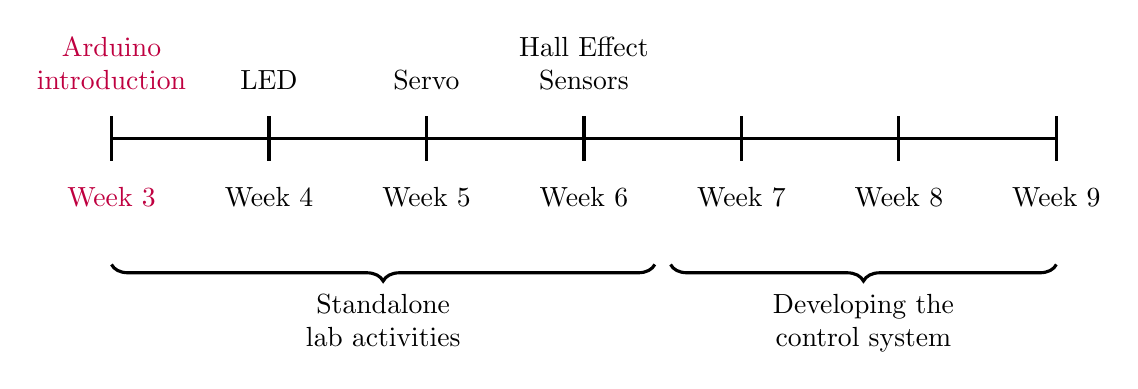
\begin{tikzpicture}[
            timeline/.style={color=black, line width=0.4mm},
            pastnode/.style={align=center, color=darkgray},
            currentnode/.style={align=center, color=purple},
            futurenode/.style={align=center, color=black}
        ]
            %line
            \draw[timeline] (-6, 0) -- (6, 0);

            % week ticks
            \foreach \x in {-6, -4, -2, 0, 2, 4, 6}{
                \draw[timeline] (\x, -0.28) -- (\x, 0.28);
            }

            % weeks (below the line)
            \node[currentnode, below] at (-6, -0.5) {Week 3};
            \node[futurenode, below] at (-4, -0.5) {Week 4};
            \node[futurenode, below] at (-2, -0.5) {Week 5};
            \node[futurenode, below] at (0, -0.5) {Week 6};
            \node[futurenode, below] at (2, -0.5) {Week 7};
            \node[futurenode, below] at (4, -0.5) {Week 8};
            \node[futurenode, below] at (6, -0.5) {Week 9};

            % activities (above the line)
            \node[currentnode, above] at (-6, 0.5) {Arduino\\introduction};
            \node[futurenode, above] at (-4, 0.5) {LED};
            \node[futurenode, above] at (-2, 0.5) {Servo};
            \node[futurenode, above] at (0, 0.5) {Hall Effect\\Sensors};

            % phases
            \draw[timeline, decorate, decoration={brace, amplitude=6pt, mirror}] (-6, -1.6) -- (0.9, -1.6);
            \node[futurenode, below] at (-2.55, -1.85) {Standalone\\lab activities};
            \draw[timeline, decorate, decoration={brace, amplitude=6pt, mirror}] (1.1, -1.6) -- (6, -1.6);
            \node[futurenode, below] at (3.55, -1.85) {Developing the \\ control system};

        \end{tikzpicture}
    \end{center}
\end{frame}

\begin{frame}{What is an Arduino?}
    \Large
    Arduino is an open-source electronics platform based on easy-to-use hardware and software. Arduino boards are able to read inputs - light on a sensor, a finger on a button, or a Twitter message - and turn it into an output - activating a motor, turning on an LED, publishing something online. You can tell your board what to do by sending a set of instructions to the microcontroller on the board. To do so you use the Arduino programming language (based on Wiring), and the Arduino Software (IDE), based on Processing.

    \begin{flushright}
        \vspace{.5em}
        \scriptsize
        \text{Source: https://www.arduino.cc/en/Guide/Introduction}
    \end{flushright}
\end{frame}

\begin{frame}{Arduino Nano Every}
    \begin{columns}
        \begin{column}{.5\textwidth}
            \begin{center}
                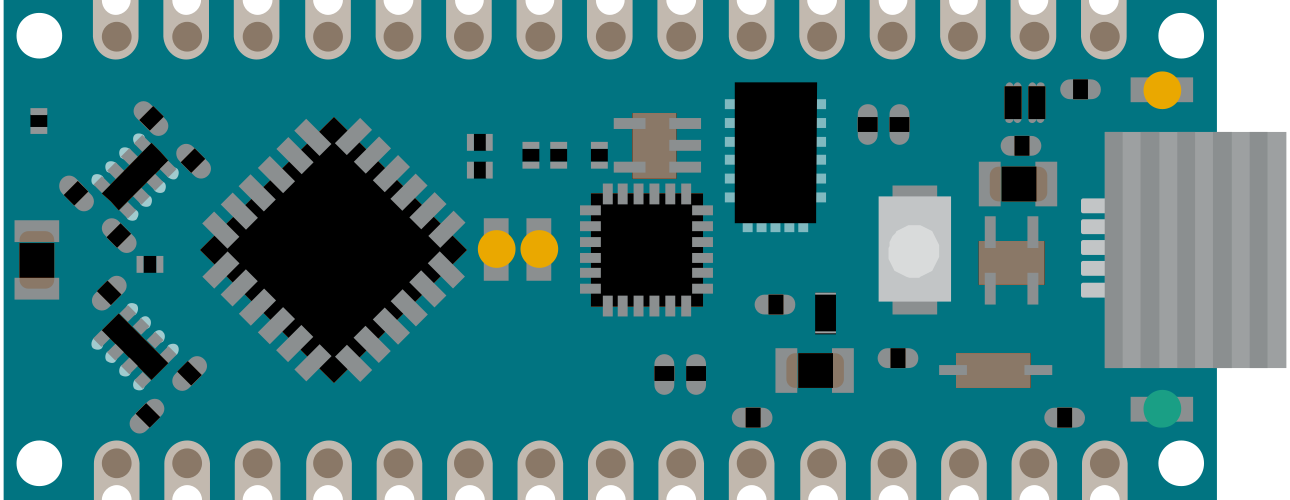
\includegraphics[width=\textwidth]{./images/nano.png}
            \end{center}
        \end{column}
        \begin{column}{.5\textwidth}
            \begin{center}
                \qrcode[hyperlink, height=4cm]{https://docs.arduino.cc/hardware/nano-every/}\\
            \end{center}
        \end{column}
    \end{columns}
    \begin{center}
        \vspace{2em}
        \scriptsize
        Source: https://docs.arduino.cc/hardware/nano-every/
    \end{center}
\end{frame}

\begin{frame}{Pinout Diagram}
    \begin{columns}
        \begin{column}{.5\textwidth}
            \begin{center}
                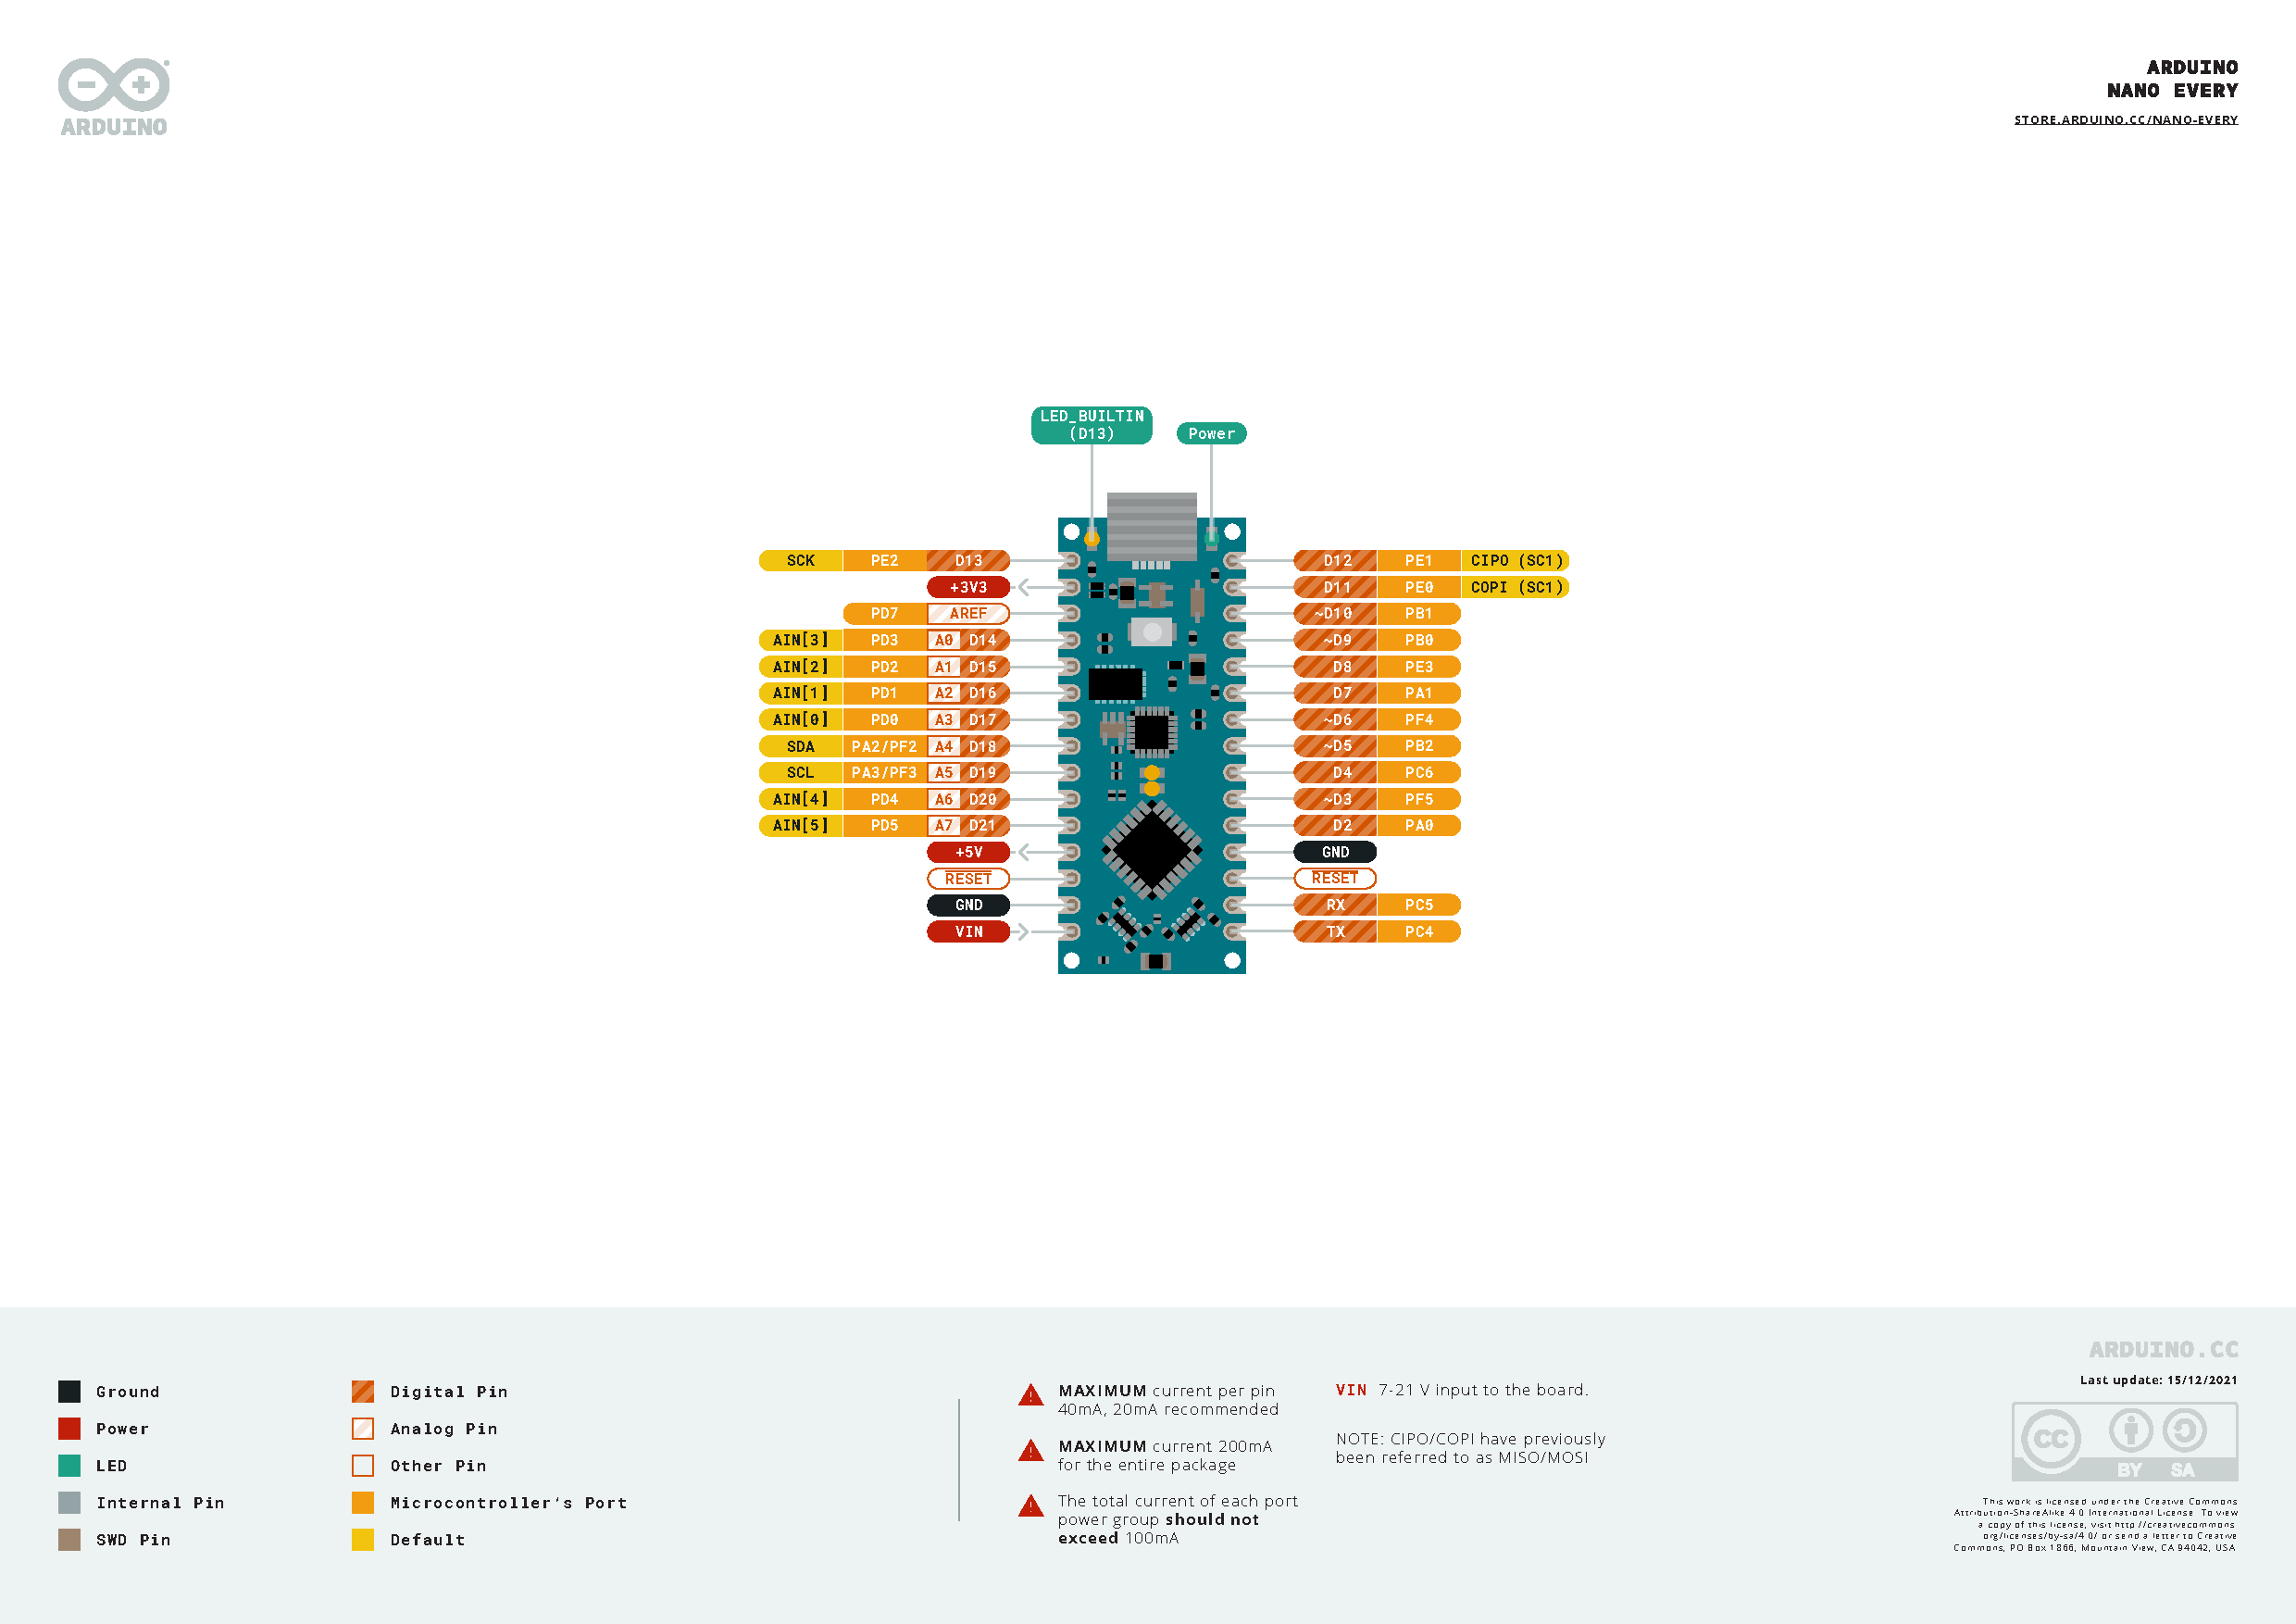
\includegraphics[width=\textwidth, trim={13cm 11cm 13cm 7cm}, clip]{./images/nano-every-full-pinout.pdf}            
            \end{center}
        \end{column}
        \begin{column}{.5\textwidth}
            \begin{center}
                \qrcode[hyperlink, height=4cm]{https://docs.arduino.cc/resources/pinouts/ABX00028-full-pinout.pdf}\\
            \end{center}
        \end{column}
    \end{columns}
    \begin{center}
        \vspace{2em}
        \scriptsize
        Source: https://docs.arduino.cc/resources/pinouts/ABX00028-full-pinout.pdf
    \end{center}
\end{frame}

%Section: Variables
\begin{frame}[standout]
    \LARGE MATLAB vs Arduino
\end{frame}

\begin{frame}{Arduino IDE}
    \begin{center}
        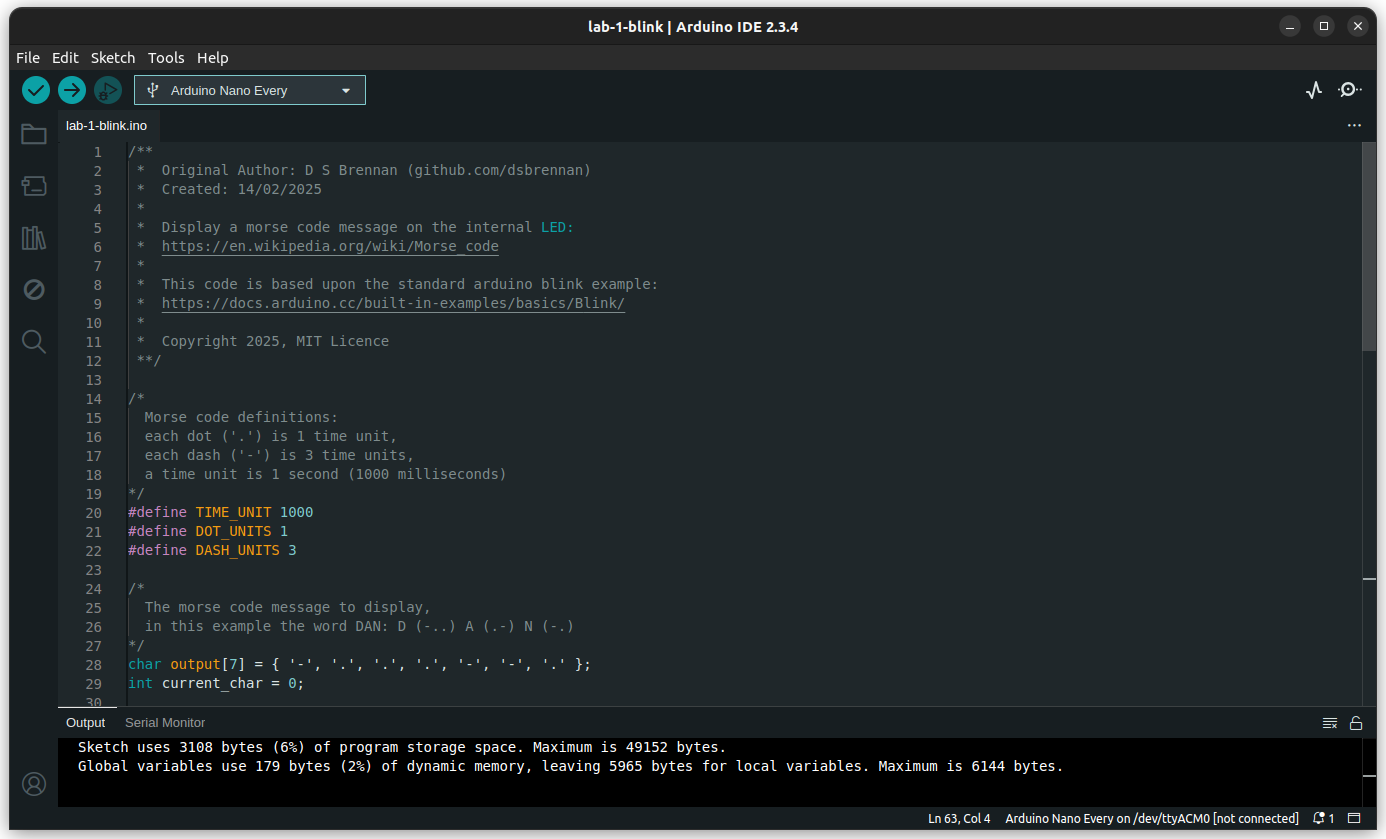
\includegraphics[width=.75\textwidth]{./images/arduino-ide.png}
        \url{https://www.arduino.cc/en/software}
    \end{center}
\end{frame}

\begin{frame}{Variables}
    \Large
    \textbf{MATLAB} is a dynamically typed language.\\
    This means you can simply declare a variable as below and MATLAB figures it out for you:\\
    \vspace{-1.5em}
    \inputminted{matlab}{./src/matlab-variable.txt}

    \vspace{1em}
    \textbf{Arduino} is a statically typed language.\\
    This means when you declare a variable, you must let Arduino know what type of data is contained within the variable:\\
    \vspace{-1.5em}
    \inputminted{arduino}{./src/arduino-variable.txt}

\end{frame}

\begin{frame}{Variables: Data Types}
    \Large
    \inputminted{arduino}{./src/arduino-data-types-numeric.txt}
\end{frame}

\begin{frame}{Variables: Data Types} 
    \Large
    \inputminted{arduino}{./src/arduino-data-types-other.txt}
\end{frame}

\begin{frame}{Variables: Qualifiers}
    \Large
    \inputminted{arduino}{./src/arduino-qualifiers.txt}
\end{frame}

\begin{frame}{Special Functions}
    \Large
    A function is a grouping of logic into a named piece of code that you can then call from somewhere else in your code.\\

    Arduino has two special functions that must exists in a Sketch before it can be compiled and uploaded to your Arduino: `setup' and `loop'.\\
\end{frame}

\begin{frame}{Minimum Sketch}
    \Large
    \inputminted{arduino}{./src/arduino-minimum.txt}
\end{frame}

\begin{frame}{Variables: Scope}
    \Large
    The scope of a variable, is which areas of the program it is valid within e.g where can it be accessed.\\

    A variable can either be within the scope of a function, or it can be within the scope of the whole program.\\
\end{frame}

\begin{frame}{Variables: Scope}
    \Large
    \inputminted{arduino}{./src/arduino-scope.txt}
\end{frame}

%Section: Conditionals
\begin{frame}[standout]
    \LARGE Control Structure
\end{frame}

\begin{frame}{Control Structure: If}
    \Large
    You will often want to control what happens in your code depending on certain conditions.\\

    The most useful control structure for our use case is an `if'. If the condition is `true', then the code within the curly brackets gets executed.\\
    \inputminted{arduino}{./src/arduino-if.txt}
\end{frame}

\begin{frame}{Control Structure: If-Else}
    \Large
    The `if' control structure can be extended with an `else'.\\

    The code within the curly brackets after the `else' gets executed if the condition is `false'.\\
    \inputminted{arduino}{./src/arduino-if-else.txt}
\end{frame}

\begin{frame}{Control Structure: If-Else-If}
    \Large
    This can be further extended to chain multiple conditions together.\\
    \inputminted{arduino}{./src/arduino-if-else-if.txt}
\end{frame}

\begin{frame}{Condition}
    \Large
    A condition is the comparison of the `left' value to the `right value'. A condition will be true if the comparison is correct.\\
    
    `$X == Y$' The X and Y value are the same\\
    `$X != Y$' The X and Y value are not the same\\
    `$X < Y$' X is less than Y\\
    `$X <= Y$' X is less than or equal to Y\\

    Conditions can be chained together by either an and ($\&\&$) or an or ($\|$).\\

\end{frame}

\begin{frame}{Condition}
    \Large
    \inputminted{arduino}{./src/arduino-condition.txt}
\end{frame}

%Section: IO
\begin{frame}[standout]
    \LARGE IO \& Interrupts\\
    \normalsize Inputs \& Outputs
\end{frame}

\begin{frame}{Pin Mode}
    \Large
    Inputs and Outputs from the Arduino are handled by the `Pin's on the board.\\

    Each Pin in numbered and can be configured as an input or an output. This decision must be made within the `setup' function of your Sketch.\\

\end{frame}

\begin{frame}{Pin: Mode}
    \Large
    The `pinMode' function sets the mode for a Pin. The first parameter is the pin number, and the second parameter is either `INPUT' or `OUTPUT'.\\

    \inputminted{arduino}{./src/arduino-io-mode.txt}
\end{frame}

\begin{frame}{Pin: Setting the output value}
    \Large
    An output pin can either have the value set to LOW or HIGH.\\

    \inputminted{arduino}{./src/arduino-io-output.txt}
\end{frame}

\begin{frame}{Pin: Reading the input value}
    \Large
    An input could change at any point. As such, we can't rely upon the value to change when we are at a certain point in the `loop' function.\\
    
    Instead, we have to `interrupt' the main `loop' function to record the value.\\

    The `interrupt' function can be called when the input value is `LOW', `CHANGE', `RISING', or `FALLING'.\\
\end{frame}

\begin{frame}{Pin: Reading the input value}
    \large
    \inputminted{arduino}{./src/arduino-io-input.txt}
\end{frame}

\begin{frame}{Additional Information}
    \Large
    \begin{center}
        I have only covered the most useful variables and structure for our use case; however, there are many more options available:\\
        \vspace{1em}
        \qrcode[hyperlink, height=4cm]{https://docs.arduino.cc/language-reference}\\
        \vspace{1em}
        \url{https://docs.arduino.cc/language-reference}
    \end{center}
\end{frame}

%Section: Lab
\begin{frame}[standout]
    \LARGE Lab 1\\
    \normalsize Communicating with the internal LED
\end{frame}

\begin{frame}{Step 1: Download and Install Arduino IDE}
    \begin{center}
        Go to \url{https://www.arduino.cc/en/software}
        \begin{tikzpicture}[
            highlight/.style={draw=purple, line width=.25mm},
        ]
            % screenshot
            \node[] at (0, 0) {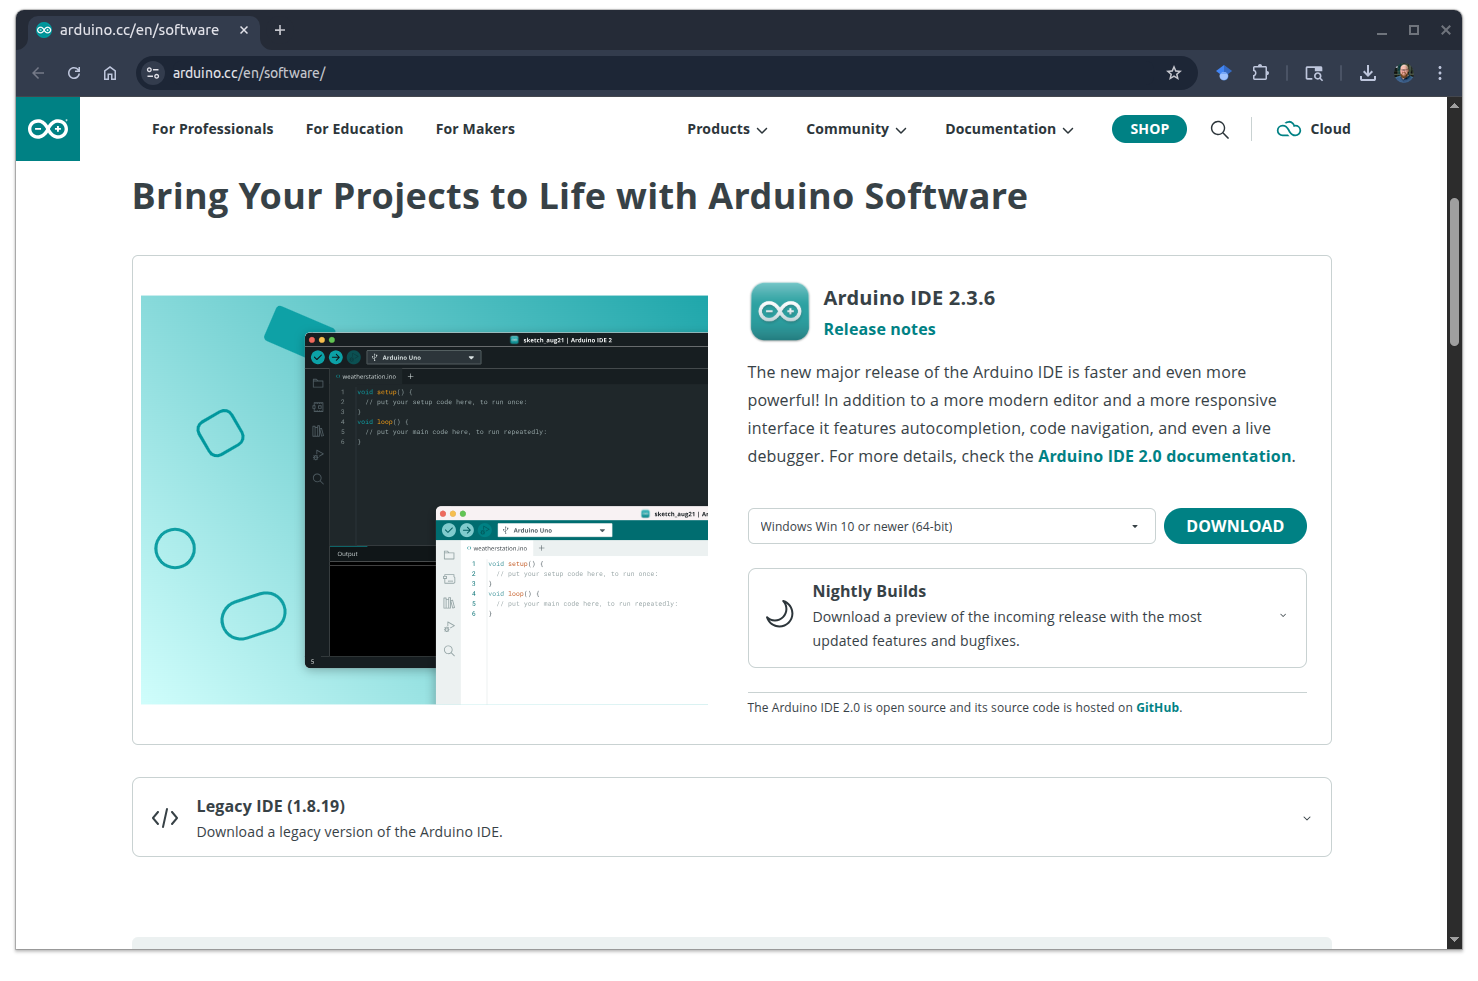
\includegraphics[width=.7\textwidth]{./images/arduino-download.png}};
            % highlight
            \draw[highlight] (0, -.5) rectangle ++(3.85, 0.5);
        \end{tikzpicture}
    \end{center}
\end{frame}

\begin{frame}{Step 2: Download Lab 1 from Blackboard}
    \begin{center}
        Login to Blackboard: \url{https://vle.shef.ac.uk/}
        \begin{tikzpicture}[
            highlight/.style={draw=purple, line width=.25mm},
        ]
            % screenshot
            \node[] at (0, 0) {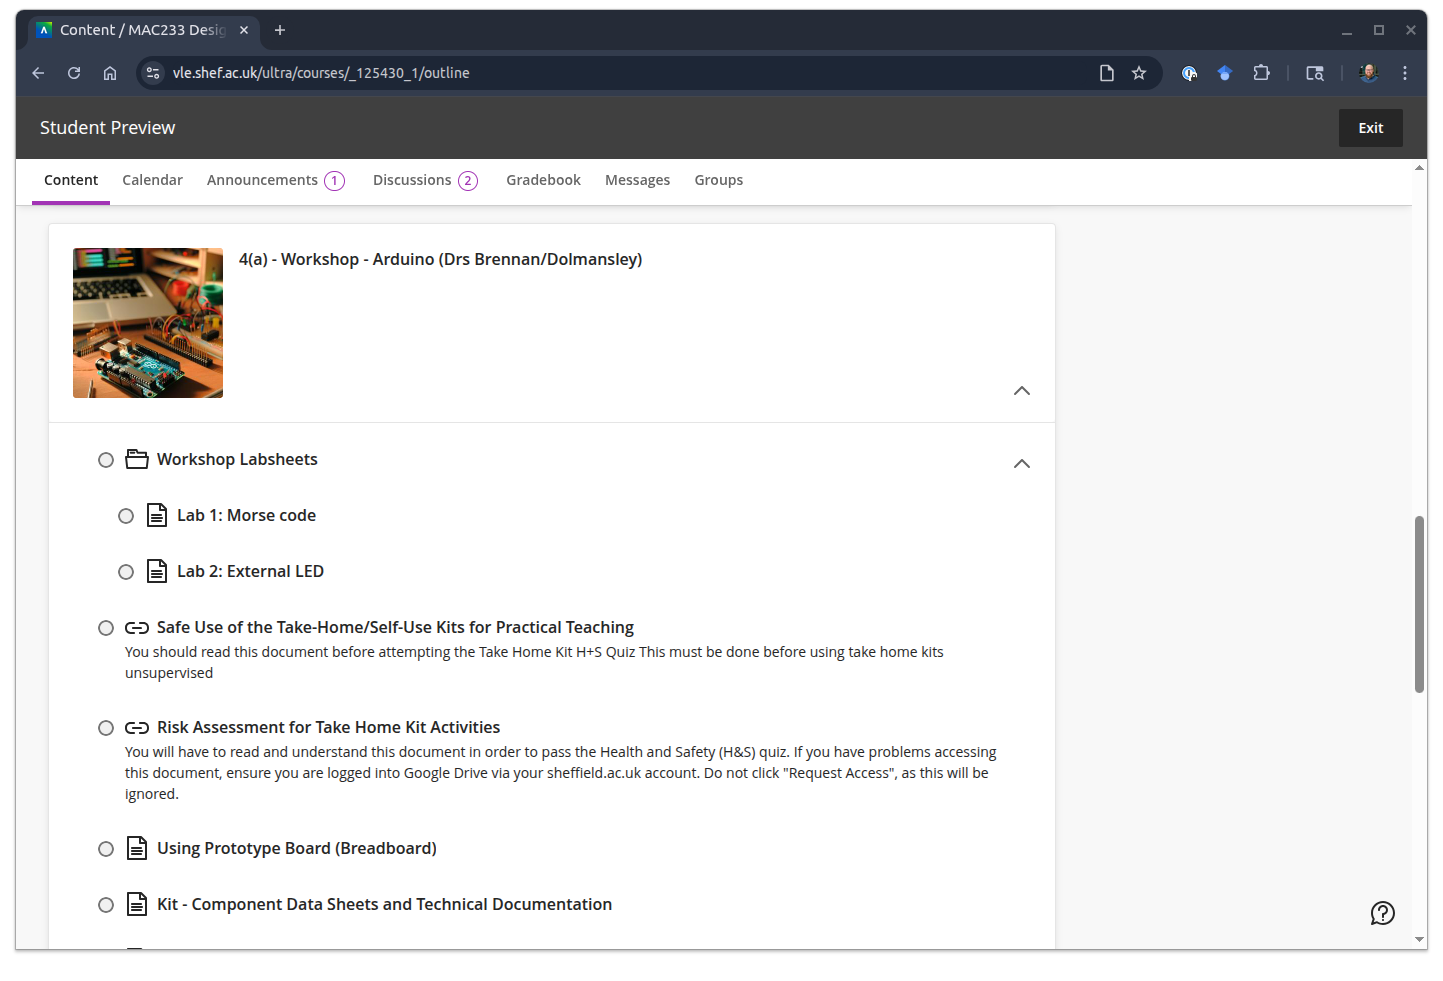
\includegraphics[width=.7\textwidth]{./images/lab-worksheet.png}};
            % highlight
            \draw[highlight] (-4.25, -.375) rectangle ++(2, 0.4);
        \end{tikzpicture}
    \end{center}
\end{frame}

\begin{frame}{Step 2: Download Lab 1 from Blackboard}
    \begin{center}
        Login to Blackboard: \url{https://vle.shef.ac.uk/}
        \begin{tikzpicture}[
            highlight/.style={draw=purple, line width=.25mm},
        ]
            % screenshot
            \node[] at (0, 0) {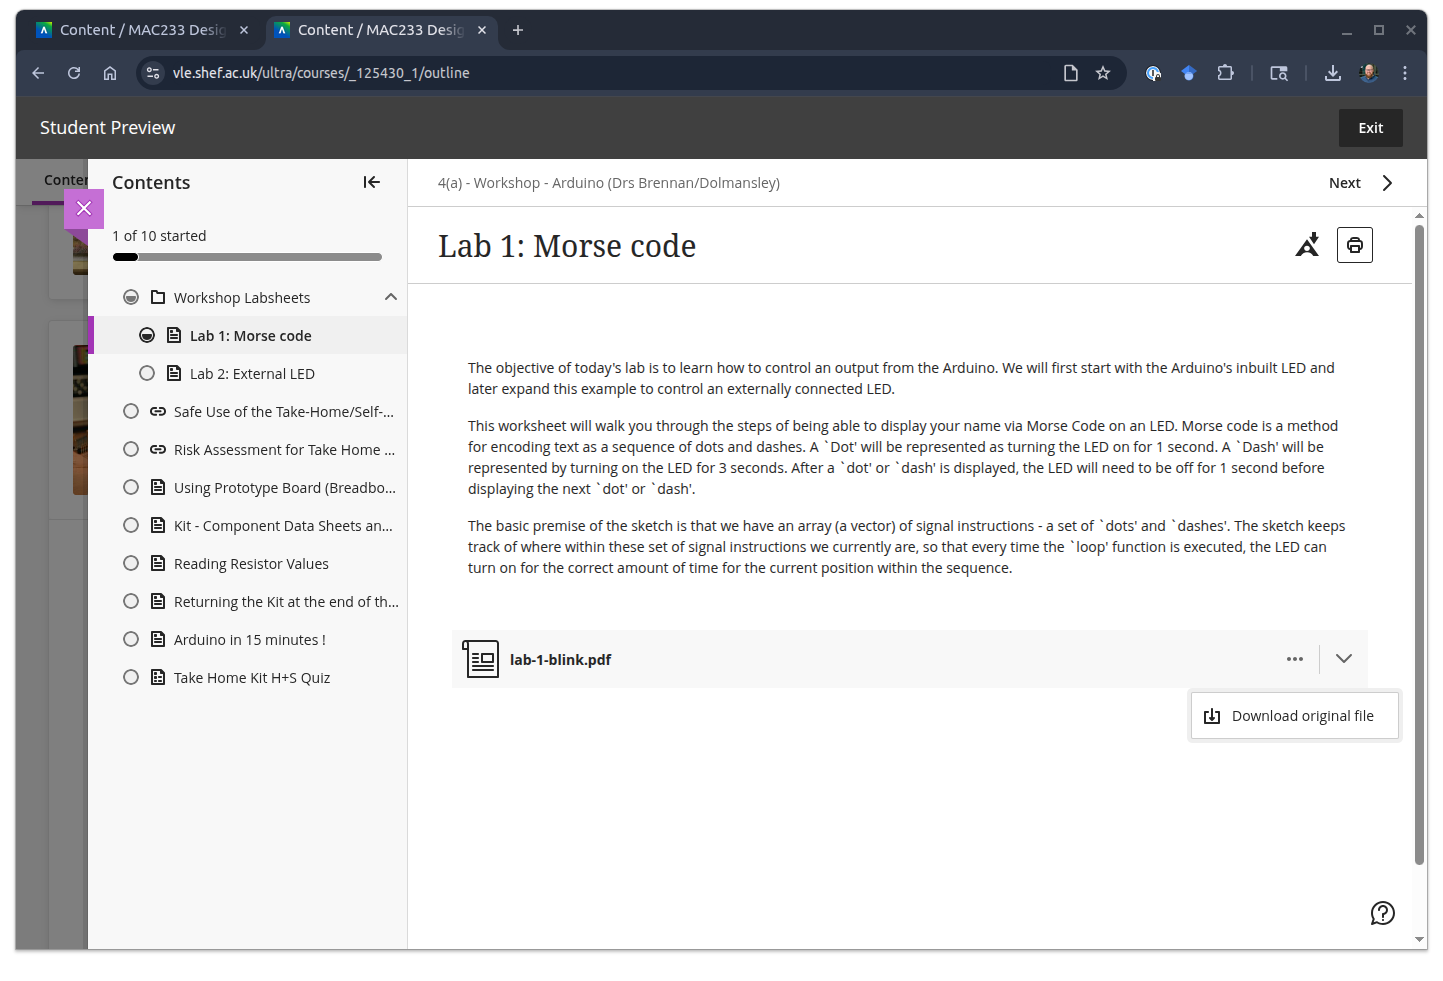
\includegraphics[width=.7\textwidth]{./images/lab-download.png}};
            % highlight
            \draw[highlight] (3.1, -1.8) rectangle ++(1.6, 0.5);
        \end{tikzpicture}
    \end{center}
\end{frame}

\begin{frame}{Step 3: Select the correct board and port}
    \begin{center}
        \begin{tikzpicture}[
            highlight/.style={draw=purple, line width=.25mm},
        ]
            % screenshot
            \node[] at (0, 0) {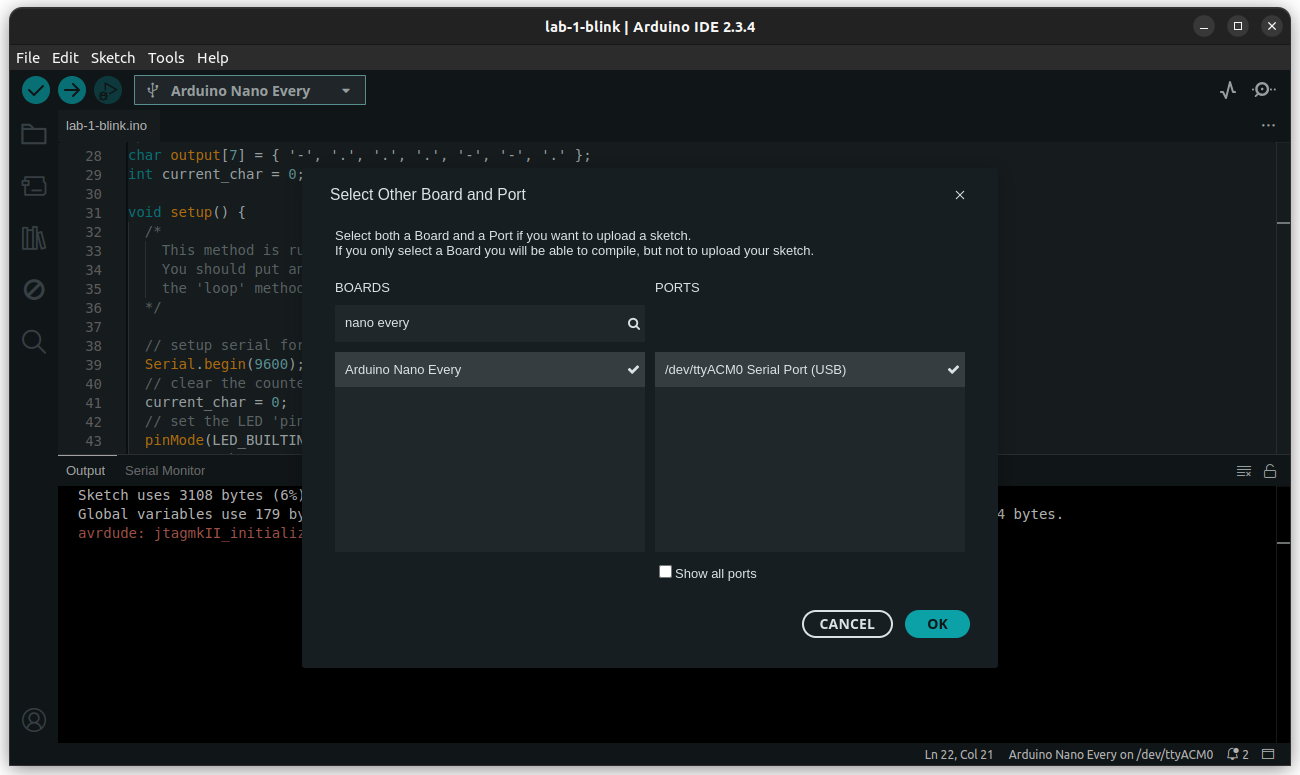
\includegraphics[width=.8\textwidth]{./images/arduino-board-selection.png}};
            % highlight
            \draw[highlight] (-4.5, 2.3) rectangle ++(2.1, 0.5);
            \draw[highlight] (-2.75, -.1) rectangle ++(2.5, 0.5);
            \draw[highlight] (0, -.1) rectangle ++(2.5, 0.5);
        \end{tikzpicture}
    \end{center}
\end{frame}

\begin{frame}{Help}
    \begin{center}
        Raise your hand and someone will come and help you.
        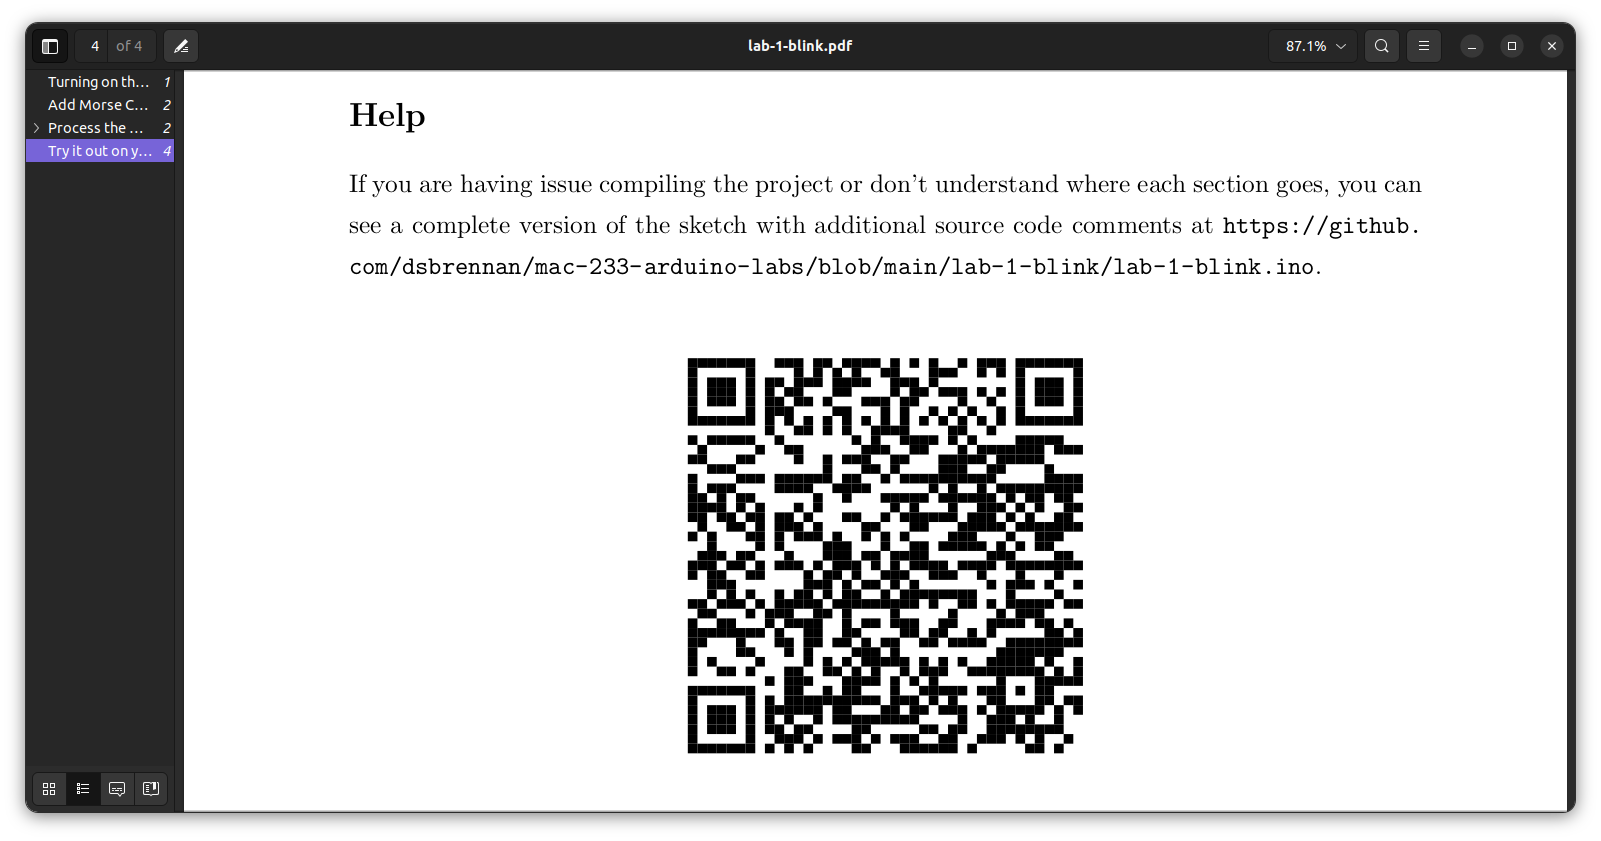
\includegraphics[width=.8\textwidth]{./images/lab-help.png}
    \end{center}
\end{frame}

\end{document}